%!TEX encoding = UTF-8 Unicode
\chapter{Einführung, Begriffserklärung und Arteneinteilung}
Im ersten Kapitel wird zuerst eine kurze Einführung zum Thema gegeben, anschließend werden die wichtigsten Begriffe vorgestellt. Danach werden zwei Unterteilungen für die Beratungsbranche vorgestellt und erläutert.
\section{Einleitung}
In Zeiten immer komplexerer und internationaler Unternehmensstrukturen, Organisation und technischer Vernetzung, ist es aufgrund der Komplexität manchmal nötig erfahrene Berater zu beauftragen. Diese können sowohl von innerhalb des Unternehmens kommen als auch von außerhalb. Mit einem anderen Blick auf das Unternehmen und einer gewissen Erfahrung können oftmals Probleme erkannt und beseitigt werden. Die Bandbreite der Beratungsleistungen, die von externen Beratern angeboten werden ist dabei sehr groß. Oft fällt es schwer die teilweise ähnlichen Begriffe zu unterscheiden und eine genaue Auswahl der benötigten Dienstleistung zu treffen. Auch die IT-Beratung als Teil der allgemeinen Beratung bietet verschiedene Dienstleistungen an. Diese reichen von reiner Konzeption der IT bis hin zum Betrieb kompletter Geschäftsprozesse (BPO). International ist der IT-Consulting Markt jedoch sehr verschieden verteilt. Wie entwickelt ist die IT-Beratungsbranche zum Beispiel in Indien? Welche Umsätze werden generiert? Gibt es genügend Fachkräfte? Welchen Einfluss hat die Arbeitskultur des jeweiligen Landes auf die IT-Beratungsbranche? Anhand eines internationalen Vergleiches versucht diese Arbeit die Fragen dieser Art zu beantworten.

\subsection*{Ziele}
Im Rahmen dieser Arbeit soll zuerst ein Überblick über die Consulting Branche als ganzes gegeben werden. Dabei werden die wichtigsten Begriffe erklärt und verschiedene Möglichkeiten der Untergliederung aufgezeigt. Anschließend wird die Beratungsart IT-Beratung genauer betrachtet und es werden wesentliche Begriffe erläutert. Ziel der Kapitel Markt, Arbeitskultur und Bildung ist es, anhand ausgewählter Aspekte, einen internationalen Vergleich der IT-Consulting Branche anzustellen. Dazu wird zuerst anhand von Teilaspekten ein theoretisches Grundgerüst geschaffen und danach ein Vergleich einer Auswahl dieser Teilaspekte durchgeführt.
\subsection*{Struktur}
Diese Arbeit soll im ersten Kapitel einen Überblick über die Unternehmensberatung geben. Dazu werden zuerst wesentliche Begriffe aus dem Beratungsumfeld definiert. Anschließend werden verschiedene Unterteilungen vorgestellt, die es ermöglichen die verschiedenen Teilgebiete weiter abzugrenzen. Es werden die BDU-Einteilung und die Lünendonk-Einteilung vorgestellt und die zugehörigen Begriffe erläutert.
Im den drei folgenden Kapiteln wird der Schwerpunkt auf das IT-Consulting gesetzt und ein internationaler Vergleich durchgeführt. Das Kapitel Markt beschäftigt sich mit der allgemeinen Marktsituation. Im Kapitel Arbeitskultur wird der Einfluss der Arbeitskultur auf die IT-Beratung betrachtet. Das Kapitel Bildung erklärt die Relevanz der Bildungssituation auf die Branche. Dabei wird in jedem Kapitel zuerst eine theoretische Betrachtung durchgeführt. Diese besteht darin den jeweiligen Aspekt (Markt, Arbeitskultur, Bildung) in verschiedene Teilaspekte zu untergliedern. Anschließend wird die Relevanz dieser Teilaspekte für das IT-Consulting betrachtet. Aufgrund zeitlicher Einschränkungen werden dann nur einige ausgewählte Teilaspekte anhand einiger ausgewählter Länder verglichen. 

\section{Consulting Begriffe}
Im Folgenden werden die wichtigsten Begriffe aus dieser Arbeit erläutert.
\subsection*{Unternehmensberatung}
Als Synonyme zur Unternehmensberatung werden häufig auch die Begriffe “Consulting”
oder “Management Consulting” verwendet. Im Duden wird Consulting als Beratung; Beratertätigkeit (besonders in der Wirtschaft) angegeben. Der Begriff Consulting ist daher vollständig eingedeutscht und es wird sich explizit auf wirtschaftliche Beratung bezogen. 
In dieser Arbeit wird sich allerdings hauptsächlich auf den Begriff Unternehmensberatung bezogen, welcher im wissenschaftlichen Umfeld eher Bestand hat.
Sowohl in der Literatur, als auch in der Umgangssprache scheint es gewissermaßen einen Konsens zu geben, was den Begriff Unternehmensberatung angeht. 
Jedoch wird der Begriff teils aus verschiedenen Perspektiven betrachtet. Häufig wird eine funktionale Perspektive als Ausgangspunkt verwendet, welche den Prozess der Unternehmensberatung als Tätigkeit beschreibt. Es gibt jedoch auch vereinzelt institutionelle Herangehensweisen zur Definition, welche die Unternehmensberatung nicht als Methode, sondern als Institution charakterisiert. Da beide Begriffe sowohl in der Literatur als auch in der Umgangssprache öfter auftauchen, soll hier ein funktionaler -und institutioneller Begriff unterschieden werden. In der nachfolgenden Arbeit wird der Begriff Unternehmensberatung im funktionalen Sinne verwendet.

\subsection*{Funktionaler Begriff}

Eine Bestätigung der Uneinheitlichkeit des Consulting-Begriffes liefert Nissen \cite[10]{nissen2007consulting}. Er verweist bereits auf die uneinheitliche Begriffsdefinition in der wissenschaftlichen Literatur. \cite[7]{ernst2002evaluation}. Die Ursache liegt laut Ernst \cite[10]{ernst2002evaluation} in der fragmentierten Forschungsgemeinschaft, welche unterschiedliche Untersuchungsziele und Abgrenzungszwecke verfolgt. 
Jedoch gibt es einen vermeintlichen Konsens, da sich die Definitionen teilweise überschneiden. Einig ist sich Literatur zumeist darüber, dass die Unternehmensberatung eine eigenverantwortliche, zeitlich befristete, auftragsindividuelle und zumeist gegen Entgelt erbrachte professionelle Dienstleistung \cite[14]{Lippold201309} ist, die durch eine oder mehrere, im allgemeinen fachlich dazu Befähigte und von den beratenen Klienten hierarchisch unabhängige Personen durchgeführt wird, mit dem Ziel zumeist betriebswirtschaftliche Problemstellungen eines Klienten zu identifizieren und zu analysieren. Dabei kann eine Handlungsempfehlung erarbeitet und dem Klienten bei der Planung, Erarbeitung der Lösung und Umsetzung geholfen werden.  \cite[15]{nissen2007consulting}
Teile dieser umfangreichen Definitionen tauchen in anderen Definition in der Literatur zumindest auf, oder charakterisieren einen dieser Merkmale. 
\subsection*{Institutioneller Begriff}

Einen institutionellen Begriff liefert Bamberger \cite[16]{bamberg2008strategische}.
Er stellt Unternehmensberatungen selbst als Organisationen dar. Sie haben Ziele, Strategien, Managementsysteme, Wertschöpfungsketten, Geschäftsprozesse, Organisationsstrukturen und eine Organisationskultur. Sie können unterschiedliche Geschäftsmodelle aufweisen. Diese Art der Betrachtung ist durchaus sinnvoll, da sich die Art der Unternehmung folglich auch auf den Prozess selbst auswirkt. Insbesondere im Vergleich verschiedener Beratungsunternehmen ist die Verwendung dieses Begriffs folglich ebenso sinnvoll.

\subsection*{Inhouse-Beratung}
Der Begriff Inhouse Consulting wird häufig auch als interne Beratung bezeichnet. \cite[150]{ReinekeBock200709}
Im Grunde genommen verfolgen die internen Beratungen die gleichen Ziele wie die externen. Die Mehrheit der Inhouse-Beratungen besteht entweder als GmbH oder selbständige Stabsstelle, die in den allermeisten Fällen direkt beim Vorstand bzw. der Geschäftsführung angegliedert ist. \cite[14]{B2_InhouseConsulting}
Es gibt dennoch einige zusätzliche Aspekte, die sich auf die interne Beratung nicht unwesentlich auswirken. Diese Aspekte begründen sich zum einen in der Entstehung von Inhouse-Beratungen. Diese haben meistens einen längeren evolutorischen Transformationsprozess hinter sich, der aus verschiedenste Sondersituationen wie Restrukturierungen, Zentralisierungen, Fusionen etc. hervorgeht. \cite[160]{Lippold201309}
Für Unternehmen mit einem Beratungsbedarf stellt sich die Entscheidungsfrage, ob eine interne Beratung etabliert oder eine externe Beratung angeheuert werden soll.
Aufgrund der unmittelbaren Nähe zum Top-Management und zu den Abteilungen gibt es natürlich einige Vorteile für eine interne Beratung hinsichtlich der Kommunikationswege.
Diese Tatsache verspricht natürlich Kosteneinsparungen und Synergieeffekte. Eine Erörterung der Vor -und Nachteile soll hier allerdings nicht erfolgen, da der primäre Fokus auf Erfassung der Daten liegt und nicht auf dessen Bewertung.

\subsection*{Externe Beratung}
Die externe Beratung ist das Pendant zur internen Beratung. Im allgemeinen Sprachgebrauch ist unter Unternehmensberatung eine externe Beratung zu verstehen. Inhouse-Beratungen bilden daher eher die Ausnahme. Externe Beratungen fungieren als Dienstleistungsunternehmen und haben häufig mehrere Kunden. Dies hat zur Folge, dass wesentlich mehr Branchen beraten werden und ein breiteres Know-How und branchenspezifisches Spezialwissen erforderlich ist. Durch die Eigenständigkeit herrscht außerdem ein höherer Wettbewerb, was wiederum einen zusätzlichen Anreiz zur Verbesserung der Beratungsqualität schafft.
Einen Spezialfall bilden hier noch die externen Beratungen, die als Tochtergesellschaften von Konzernen fungieren und beispielsweise Dienstleistungen, wie  die Verwaltung der eigenen IT, an eigene eigenständige externe Beratung auslagern. ( Beispiel Deutsche Telekom AG, 01.11.2011)


\section{Einteilung in Beratungsarten}
Die Einteilung eines praktischen Gebietes, wie es die Beratung darstellt, ist oftmals schwierig. Besonders einheitliche und eindeutige Definitionen zu den Einteilungen sind oftmals nicht beschrieben und nicht scharf abgegrenzt. Trotzdem sollte aus wissenschaftlicher Sicht der Versuch einer Einteilung unternommen werden um zumindest eine grobe Abgrenzung zu realisieren.

\subsection{BDU-Einteilung}
In einigen Literaturquellen \cite[54]{Lippold201309},\cite[4]{nissen2007consulting} wird die so genannte BDU-Einteilung der Beratungsfelder verwendet (BDU: Bund Deutscher Unternehmensberater). Der BDU verwendet die Einteilung als Grundlage für seine statistischen Erhebungen. Deswegen ist sie trotz ihrer Schwächen (nächster Abschnitt) relevant.
Die BDU Einteilung unterteilt in: Strategieberatung, Organisations- und Prozessberatung, IT-Beratung und Human-Ressource Beratung. Eine klare Definition der einzelnen Bestandteile der 4 Bereiche wird vom BDU nicht angegeben. Einige Kritikpunkte an dieser Einteilung werden von (\cite[54]{Lippold201309} aufgeführt. So wird kritisiert, \glqq [...] dass sich Organisations- und Prozessberatung nicht oder nur sehr schwer von der IT-Beratung trennen l\"asst \grqq. (\cite[54]{Lippold201309} . Dies lässt sich verstehen indem man sich die Abhängigkeiten von IT und Organisation verdeutlicht. Eine klare Einteilung in diese zwei Bereiche erscheint schwierig, da die IT von der Organisation wesentlich abhängt und auch manchmal die Organisation von den IT Möglichkeiten. Eine weitere „wesentliche Schwäche“ (\cite[54]{Lippold201309}  wird deutlich wenn man das 4. Beratungsfeld die Human Ressource betrachtet. Laut (\cite[54]{Lippold201309} wird sie als einzige der funktionalen Beratungsarten erwähnt. Die Einteilung in funktionale Beratungsargen wird jedoch in dieser Arbeit nicht beschrieben. Sie kann zum Beispiel bei Nissen nachgelesen werden. Die anderen funktionalen Beratungsarten (z.B.Marketingberatung, Controlling-Beratung, Logistik- Beratung etc.) finden überhaupt keine Erwähnung.
Trotz dieser wesentlichen Schwächen sollen hier eine kurze Erklärung der einzelnen Beratungsfelder folgen. Weiterhin wird der Versuch einer Abgrenzung der Begriffe untereinander unternommen. Da die Human-Ressource Beratung zu den funktionalen Beratungsfelder gehört, werden im folgenden nur die 3 verbleibenden Kernberatungsfelder erklärt. Auf eine Erklärung der funktionalen Beratungsfelder wird verzichtet. 

%\subsubsection*{Strategieberatung Version von Sebastian}
%Laut (B4, S.60) betrifft die Strategieberatung den „Kernbereich aller Unternehmensaktivitaeten, die Unternehmensstrategie“ . Zu den wichtigsten Ansprechpartnern zählen daher „Vorstände und Geschäftsführer“ . Außerdem ist die Unternehmensstrategie „mit großer Unsicherheit behaftet“ . Daher gilt es „[...] zu antizipieren“.  Gegenstand der Strategieberatung sind „Zielkunden,Leistungsversprechen und Geschäftsmodelle“. Dabei werden „verschiedene Auffassungen über die Weiterentwicklung des Unternehmens“ diskutiert.
%Die Anlässe für die Strategieberatung sind vielfältig. Es kann um das Neuentwickeln,Ändern,Weiterentwicklung, Verifizierung und Umsetzung von Strategien handeln.
%Die Aufgaben der Strategieberatung sind vielfältig dazu zählen z.B. Bestandsaufnahme,Problemerkennung und Identifizierung ,Auswahl relevanter Informationen, Hypothesenentwicklung, Analyse und Bewertung, Szenarioentwicklung, Entscheidungsvorbereitung, Umsetzungsplanung.

\subsubsection*{Strategieberatung}
Auch der Begriff Strategieberatung kann genauso wie der Beratungsbegriff institutionell und prozessorientiert betrachtet werden.
Nachfolgend werden beide Definitionsvarianten erklärt. 
\paragraph*{institutioneller Begriff}

 Strategieberatung ist eine Art der Unternehmensberatung, die sich auf strategische, immer zukunftsgerichtete Fragen eines Unternehmens spezialisiert. Dazu gehören: ``Überprüfung, Weiterentwicklung oder Neuentwicklung von Zielrichtungen, Konzepten und Maßnahmen einschließlich der Gestaltung gesamthafter Geschäftsmodelle``\cite [424]{ReinekeBock200709}. Als Gegenstand für Strategieberatung laut Schneider wird einerseits das Unternehmensumfeld(z.B. Märkte, Technologie,Wettbewerb usw.) und anderseits die Zielsetzung des Unternehmens verstanden. Wichtig ist dabei eine Strategie zu entwickeln, um die Bereitschaft zum strategischen Handeln und ein breites Spektrum fachlicher Kompetenzen zu erfordern \cite [424]{ReinekeBock200709}.

\paragraph*{prozessorientierter Begriff}

 Bamberger und Wrona bezeichnen Strategieberatung als strategische Unternehmensberatung, die als eine Art der Beratung zur strategischen Unternehmensführung interpretiert ist \cite[4]{BambergerWrona201205}. Basis für diese Definition im Vergleich zum oben stehenden Begriff bildet die strategische Unternehmensführung. Unter strategischer Unternehmensführung versteht man solche Prozesse wie ``Entscheidungen, Handlungen und Interaktionen, die sich auf die Entwicklung von Erfolgspotenzialen beziehen`` \cite[4]{BambergerWrona201205}.
 In diesem Fall bildet die Grundlage für Strategieberatung ``die Bestimmung von Zielen (wie im institutionellem Begriff ), Strategien, grundlegendem Ressourceneinsatz und Grundsätzen auf der Ebene der Gesamtunternehmung ``\cite[4]{BambergerWrona201205}.

In beiden Definitionen gibt es eine leicht ersichtliche  Gemeinsamkeit, nämlich dass die Strategieberatung eine Beratungsdienstleistung für ein bestimmtes Unternehmen in strategischen Fragen ist. 
Was  für ein Unternehmen steckt hinter dem Begriff der Strategie im Detail? Eine verbreitete Definition für die Strategie stammt vom kanadischen Managementforscher Henry Mintzberg.


\paragraph*{Eigene Synthese unter Verwendung der Strategie-Definition von Henry Mintzberg} 
Mintzberg definiert die Strategie des Unternehmens mit Hilfe von den fünf untenstehenden Merkmalen - den sogenannten “5 p’s of strategy”.
Strategie ist im Sinne dieser Definition:
\begin{itemize}

\item plan (Plan um Geschäftserfolg zu erreichen)
\item pattern (Mustern um die Regelmäßigkeiten im Unternehmen zu erfassen)
\item position (Markt- und Wettbewerbsposition)
\item perspective (Perspektive und Weltanschauung)
\item ploy (Spielzeug, Auswahl der taktische Maßnahmen) 
\end{itemize}
beschrieben \cite{5Ps}.

Die Strategieberatung findet einen passenden Lösungsansatz für die Probleme, die in all diesen Merkmalen entstehen können.


\subsubsection*{Organisations- und Prozessberatung}

\paragraph*{Gemeinsame Definition}
Laut \cite[63]{Lippold201309} beschäftigt sich die Organisations- und Prozessberatung mehr \glqq mit Fragen der Aufbau- oder Ablauforganisation sowie Prozessen\grqq und setzt dabei auf eine \glqq bestehende oder neu erarbeitete Strategie eines Unternehmens auf \grqq. Das Ziel \glqq dabei ist die Leistungs- und Anpassungsfähigkeit der Kundenunternehmen durch die Gestaltung oder Neugestaltung der Strukturen und Prozesse zu verbessern \grqq. Es geht darum Strukturen und Prozesse \glqq effektiver und/oder effizienter \grqq zu gestalten. Im Gegensatz zur Strategieberatung bewegt sich die Organisations- und Prozessberatung daher eher auf der Umsetzungsebene obwohl eine Abgrenzung generell schwer fällt. \cite[63]{Lippold201309} unterscheidet außerdem verschiedene Arten der Organisations- und Prozessberatung.

Es wird unterschieden in die gutachterliche Beratung die \glqq vornehmlich dem Wissenstransfer und der Erkenntnisvermittlung \grqq dient. So können \glqq wissenschaftliche Erkenntnisse in das Kundenunternehmen transferiert werden.\grqq . Die Expertenberatung dient dazu einen \glqq Problemlösungsprozess \grqq anzustoßen. Im Gegensatz zur gutachterlichen Beratung wird hier auch die Umsetzung beachtet. Die dritte Art ist die Organisationsentwicklung. Dort ist der Berater \glqq eher passiv\grqq. 
Die Mitarbeiter des Unternehmens sollen nach einer Anlernphase ihr Unternehmen selbst \glqq entwickeln \grqq . 
Die letzte Art, die systemische Beratung ist aus der neueren Systemtheorie entstanden. Der Kunde wird unterstützt \glqq bei seiner Selbstreflexion\grqq. 

\paragraph*{Einzelne Definition beider Begriffe}
Die Begriffe Organisationsberatung und Prozessberatung werden in der Literatur auch teilweise einzeln und eigenständig definiert.

In \cite[28]{MuellerNagel} findet man eine Definition für Organisationsberatung (eine Definition für Prozessberatung fehlt) . Demnach ist Organisationsberatung eine Beratung die \glqq  sich auf menschliche Kollektive bezieht, die ihr Verhalten auf gewisse Weise miteinander abstimmen (koordinieren) und so eine Handlungsrealität herstellen, die – mehr oder weniger – funktional ist. Diese Kollektive befinden sich im ständigen Prozess des Organisierens und versuchen so Probleme zu lösen, die zur Aufrechterhaltung ihres Daseinszwecks gelöst werden müssen. Immer wieder wird aber entweder genau dieser Prozess zum eigentlichen Problem, das dann mit externer Hilfe in Form von Organisationsberatung gelöst werden soll, oder der Daseinszweck steht in Frage und drängt nach neuen Antworten.
\grqq Hier wird der Begriff aus dem sozialen Kollektiv hergeleitet, dass einen bestimmten Daseinszweck besitzt, der sich aus bestimmten Problemen ableitet.

In \cite[9]{HBProzess} wird der Begriff Prozessberatung näher beschrieben. Demnach sind Prozessberater nicht mit Fachberatern zu verwechseln die Geschäftsprozesse optimieren und Ablauforganisation umgestalten. Der Anspruch des Managements wird als \glqq Culture follows strategy \grqq beschrieben. Das heißt, die Unternehmenskultur richtet sich an der Unternehmensstrategie aus. Laut \cite[9]{HBProzess} ist Veränderung oftmals ein unendlich verlangsamer Prozess. Dadurch kann es passieren das die Unternehmenskultur die Strategie besonders am Anfang verdrängt oder überlagert und damit die Veränderung erschwert. Die Prozessberatung behandelt dieses Spannungsfeld zwischen Unternehmenskultur und Unternehmensstrategie.
Der Begriff Unternehmenskultur wird auf \cite[ Seite 9]{HBProzess} beschrieben. Er ist mit einem tieferen Verständnis der Organisation verbunden. Einige
Ansätze stammen z.B. aus der Systemtheorie (Luhmann), der Kommunikationstheorie (Watzlawick) und dem Konstruktivismus. Zur Unternehmenskultur gehören z.B. bestimmte Artefakte wie Logos, Gebäudearchitektur oder Bürausstattung. Die Geistige Manifestation einer Organisation findet man z.B. in bestimmten Normen, Werten und Einstellungen oder in bestimmten \glqq Mythen oder Sagen \grqq. Solche Mythen können sich z.B. um die Gründung oder den Gründer eines Unternehmens ranken. Weiterhin wird die Kultur durch bestimmte Rituale, Zeremonien und Witze beeinflusst. So kann z.B. die Abhaltung von Meetings einem bestimmten Ablauf unterliegen, der die Unternehmenskultur beeinflusst.

Die Beschreibung der Prozessberatung hat offensichtliche Ähnlichkeiten mit der systemischen Beratung und der Organisationsentwicklung aus der gemeinsamen Definition (vorheriger Abschnitt). Beide versuchen ein tieferes Verständnis des Unternehmens zu erlangen und basieren auf psychologischen / soziologischen Theorien. Dadurch wird der Mensch im Unternehmen in den Mittelpunkt gestellt.
Die Definition für Organisationsberatung basiert auch auf \grqq menschlichen Kollektiven \glqq und ist demnach ähnlich einzuordnen.
Die gemeinsame Definition enthält noch eine weitere Komponente. Dort wird auch die Optimierung von Geschäftsprozessen und der Ablauforganisation mit eingeschlossen. Die gemeinsame Definition ist demnach umfassender und soll für diese Arbeit weiter verwendet werden. 


\subsubsection*{IT-Beratung}
	\paragraph*{Grund für den Zuwachs von IT-Beratung}
		Ein wesentlicher Grund für den starken Wachstum von IT-Beratungsleistungen liegt in der breiten Verbreitung der Informationstechnologie in Unternehmen. Zahlreiche Statistiken und Studien bestätigen, dass der Einsatz von modernen IT-Technologien die Arbeitsproduktivität erhöht und Geschäftsmodelle im Unternehmen automatisiert und verbessert. Rund 60\% der Beschäftigten in Deutschland  erledigen ihre Arbeit am Computer \cite{IreneBertschek.2011}.
		Der Fachbereich IT hilft heute nicht nur bei der Optimierung der Geschäftsprozesse, sondern ist als Business Partner bei erfolgreichen Unternehmen zu verstehen. Denn automatisierte Geschäftsprozesse auf Basis moderner Technologien wie Social Media, RFID, Big Data oder Cloud  ermöglichen es dem Betrieb, seine Positionierung weiter auszubauen.
		Aber nur blinde Investition in neue Technik führt nicht zum Geschäftserfolg. Viel wichtiger ist es zu wissen an welcher Stelle im Unternehmen, welche Technik eingesetzt werden soll um die Geschäftsprozesskette zu optimieren. IT-Technik ist dabei ein bedeutender Wertschöpfungsfaktor zum Zweck der Prozessverbesserung.
		Dadurch wird ersichtlich wie groß die Rolle von IT-Beratungsleistungen heutzutage  für moderne Unternehmen ist. 
		
		Ein wesentlicher Baustein dieser Ausarbeitung liegt daran, den Begriff der IT-Beratung  zu definieren sowie die Abgrenzung zur klassischen Unternehmensberatung und zu den anderen Beratungsarten zu klären.
		Genauso wie der Begriff “Consulting” ist der Begriff “IT-Consulting” vollständig eingedeutscht und beschreibt direkt auf die IT-Beratung. Beide Begriffe: “IT-Consulting” und “IT-Beratung” werden in dieser Arbeit als Synonyme verwendet.\\
		\paragraph*{Definition des Consultings}
		\textbf{IT-Consulting als prozessbezogene Beratungsart mit Fokus auf Systementwicklung und -integration}\\
			``'IT-Beratung ist Consulting von Unternehmen bei der Gestaltung von Prozessen, die durch Informationstechnologie (IT) unterstützt werden, sowie bei der Einführung von neuen IT-Systemen und -Anwendungen. Darüber hinaus unterstützen viele IT-Consultants die Unternehmen auch in den Bereichen Systementwicklung und -integration.'' \cite[208]{ReinekeBock200709}\\
			
		\textbf{ IT-Consulting als  projektbezogene Unterart des Consultings im IT-Umfeld}\\
			``'Unter IT-Consulting wird die professionelle Beratung von Unternehmen und Projekten bei der Entwicklung, Installation und Weiterführung von IT-Systemen verstanden. In Deutschland wird IT-Consulting auch als IT-Beratung bezeichnet [...]. Im Allgemeinen zählt man den Bereich IT-Consulting zur Wirtschaftsbranche der Unternehmensberatung.''
			\cite{statistaITCons}
		\paragraph*{Zusammenfassung} 
					Auf den ersten Blick kann man leicht den Begriff IT-Beratung bestimmen. IT-Beratung ist eine Beratung von Unternehmen in Fragen der Informationstechnologie.Die Probleme beginnen bereits bei der Definition von des Begriffes IT (Informationstechnologie). Informationstechnologie ist ein umfassendes Thema mit vielen Dienstleistungen (Integration von individueller Software, Customizing von Standardsoftware usw.), die für die IT-Beratung sinnvoll sind. Ziel ist dabei die Optimierung von Geschäftsprozessen und IT-Infrastruktur mit Hilfe von IT.
			Ein weiterer Aspekt, der für für den einheitlichen Begriff der IT-Beratung ein Hinderniss ist, verbirgt sich hinter der Klassifikation einer Beratung. Es lassen sich sehr viele Beratungsthemen unterscheiden: %Grafik dafür bilden
			 ``Geschäftsstrategien und -optimierungen, Personalausbildung, Prozessgestaltung und Prozessverbesserung, Systemimplementierung, Organisationsberatung, Sektor- und branchenorientierte Beratung, Markt- und Rechtsberatung sowie Spezialthemen wie
			Regulierung/Deregulierung,  Privatisierung oder Kulturanalyse und -anpassung, Prozessberatung und  interkulturelle Beratung'' \cite[37]{ReinekeBock200709}.
			Darüber hinaus unterstützen viele IT-Consultants die Unternehmen auch in den Bereichen Systementwicklung und -integration. Dabei orientieren sich die Berater stark an Modellen und Methoden der (Wirtschafts-) Informatik \cite{InfTag2011}.
			

\subsection{Lünendonk Systematik}
Eine weiterer Unterteilungsversuch für die Consulting Branche wurde von der Marktforschungsfirma Lünendonk GmbH verfasst.
Diese Systematik wird auch in der wissenschaftlichen Literatur \cite[56]{Lippold201309} verwendet. Lünendonk veröffentlicht
auch die sogenannten Lünendonk-Listen. Diese zeigen im Bezug auf Deutschland eine Art Topliste der besten Firmen (bezogen auf bestimmte Kriterien).
Die Listen sind auf der Website der Firma im Shop kostenlos herunterladbar \cite {topBITP} . Weiterhin verkauft Lünendonk in diesem Shop verschiedenste Studien u.a.
auch zu IT Consulting Themen.

\begin{figure}[H]
\center
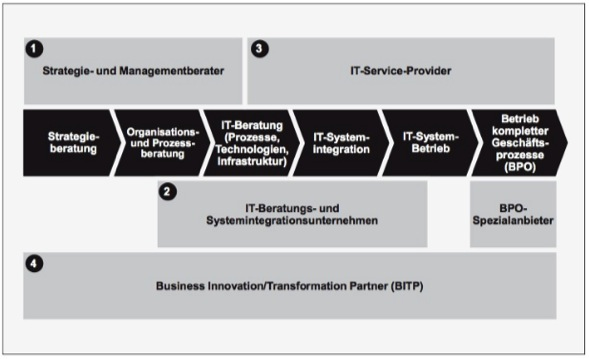
\includegraphics[width=13cm]{./images/luene.jpg}
\caption{Die Lünendonk-Systematik}
\end{figure}

Die für diese Arbeit relevante Systematik stammt aus: \cite[56]{Lippold201309}. Sie unterteilt den IT Beratungsprozess in 6 Teile :  Strategieberatung ,Organisations- und Prozessberatung, IT-Beratung (Prozesse, Technologien, Infrastruktur), IT-Systemintegration, IT-System-Betrieb, Betrieb kompletter Geschäftsprozesse (BPO). Je nach der Abdeckung dieser 6 Prozesse werden dann die verschiendenen Firmen der Branche zugeordnet. So beschäftigt sich die Strategieberatung nach Lünendonk fast nur mit Strategieberatung und Organisations- und Prozessberatung. Es existiert auch noch eine kleine Überlappung mit der IT-Beratung d.h. ein Teil der Strategieberatungen beschäftigt sich auch damit. Die 2. Kategorie IT-Beratungs und Systemintegrationsunternehmen ist eher technisch orientiert, berät aber aufgrund der Abhängigkeiten von Organisations- und Prozessberatung und der anschließenden IT Beratung auch im ersten Bereich mit. Die oben erwähnten Lünendonk Listen greifen auf diese Systematik zurück und präsentieren die jeweiligen \glqq Toplisten \grqq für diese Unternehmensarten. Die Lünendonk Systematik könnte man als zu IT-Lastig kritisieren \cite[56]{Lippold201309} . Für die vorliegende Arbeit ist sie aber aufgrund des gewählten Schwerpunktes ``IT- Consulting'' gut geeignet.

\paragraph*{Full-Service-Provider}
Der Begriff Full-Service wird in der Literatur nicht einheitlich bezeichnet. Es gibt für den betreffenden Sachverhalt mehrere ähnliche Begriffe, welche zum Teil weiter gefasst sind und andere Aspekte enthalten. Der begriff der am häufigsten in der Literatur auftritt ist der so genannte `` Full-Service-Provider'' .
Der sog. \glqq Full-Service-Provider \grqq zielt darauf ab die kompletten Anforderungen eines Kunden-Teilsegmentes abzudecken. \cite[124]{WeillVitale200106}. Dies beinhaltet folglich das gesamte Spektrum von der Strategie bis zur Umsetzung. Da Full-Service-Provider eine Komplettlösung anbieten, schließt das natürlich die Leistungen eines Content, Application und Service Providers mit ein. \cite[83]{Thalmann200708}
Es wird in diesem Zusammenhang auch die Bezeichnung Business Innvoation / Transformation Partner (BITP) verwendet, welche wiederum mit dem Begriff BPO (Business Process Outsourcing) verwandt ist. Hier liegt der Schwerpunkt vor allem auf einer langfristigen und strategischen Übernahme von ganzen Unternehmens -oder Produktsegmenten. \cite[163]{Pohland200908}\\ Häufig ist dort aufgrund der Umsetzungsnähe ein großer IT-Anteil aufzufinden. Aufgrund dessen fallen einige der Unternehmen, die sich als Full-Service-Provider bezeichnen, auch in die Gruppe der BITP. Dies lässt sich an den einschlägigen Lünedonk-Rankings beobachten. Dort gibt es Unternehmen, die sowohl im Lünedonk Top 15 Ranking für BITP auftauchen, als auch im Top-25-Ranking der IT-Beratungen.\cite {topBITP} \cite {topITB}

\paragraph*{Business Prozess Outsourcing }
Generell gibt es keinen Konsens zur Begriffsdefinition von Business Prozess Outsourcing (BPO). 
Einen betriebswirtschaftlichen Begriff liefert Tüfekciler:
BPO beschreibt den Transfer des Management und der Durchführung ein oder mehrerer kompletter Prozesse oder Geschäftsbereiche.  \cite[14]{tuefekciler2011human}
Häufig hört man den Begriff BPO im Zusammenhang mit IT-Prozessen. 

Eine Zusammenfassung als Liste mit wesentlichen Merkmalen aus mehreren IT-orientierten BPO Begriffsansätzen, liefert Mauchle \cite[6]{mauchle2012business}:
\begin{itemize}
\item Vertragliche Vereinbarung zwischen den beteiligten Parteien
\item Auslagerung von spezifischen Prozessen an ein anderes Unternehmen oder einen anderen Unternehmensbereich
\item Übergang der operativen Kontrolle und Prozesssteuerung
\item hohe IT-Intensität
\end{itemize}
Mauche versteht unter dem Begriff Business Prozess Outsourcing eine vertraglich geregelte Auslagerung eines typischerweise IT-intensiven Geschäftsprozesses an einen externen Dienstleister, welcher den Prozess fortan unter eigener operativer Steuerung und Kontrolle ausführt.
\cite[3]{mauchle2012business}

Typische BPO-Prozesse laut Halvey sind Unternehmensbereiche wie: Finanzen und Buchhaltung, Investitionsverwaltung, Personalverwaltung und Logistik. Aber sowohl schmalere- als auch noch breitere ausgelagerte Funktionsbereiche, als die genannten typischen, werden in der Literatur als BPO-Bereiche bezeichnet. \cite[4]{halvey2007business}
 







